% -*- latex -*-
%%%%%%%%%%%%%%%%%%%%%%%%%%%%%%%%%%%%%%%%%%%%%%%%%%%%%%%%%%%%%%%%
%%%%%%%%%%%%%%%%%%%%%%%%%%%%%%%%%%%%%%%%%%%%%%%%%%%%%%%%%%%%%%%%
%%%%
%%%% This text file is part of the source of 
%%%% `The Art of HPC, vol 1: The Science of Computing'
%%%% by Victor Eijkhout, copyright 2012-2022
%%%%
%%%% This book is distributed under a Creative Commons Attribution 3.0
%%%% Unported (CC BY 3.0) license and made possible by funding from
%%%% The Saylor Foundation \url{http://www.saylor.org}.
%%%%
%%%%
%%%%%%%%%%%%%%%%%%%%%%%%%%%%%%%%%%%%%%%%%%%%%%%%%%%%%%%%%%%%%%%%
%%%%%%%%%%%%%%%%%%%%%%%%%%%%%%%%%%%%%%%%%%%%%%%%%%%%%%%%%%%%%%%%

Molecular dynamics is a technique for simulating the atom-by-atom
behavior of molecules and deriving macroscopic properties from these
atomistic motions.  It has application to biological molecules such as
proteins and nucleic acids, as well as natural and synthetic molecules
in materials science and nanotechnology.  Molecular dynamics falls in
the category of particle methods, which includes N-body problems in
celestial mechanics and astrophysics, and many of the ideas presented
here will carry over to these other fields.  In addition, there are special
cases of molecular dynamics including ab initio molecular dynamics where
electrons are treated quantum mechanically and thus chemical reactions
can be modeled.  We will not treat these special cases, but will instead
concentrate on {\em classical} molecular dynamics.

The idea behind molecular dynamics is very simple:  a set of particles
interact according to Newton's law of motion, $F=ma$.  Given the
initial particle positions and velocities, the particle masses and other
parameters, as well as a model of the forces that act between
particles, Newton's law of motion can be integrated numerically
to give a trajectory for each of the particles for all future (and past)
time.  Commonly, the particles reside in a computational box with 
periodic boundary conditions.

A molecular dynamics time step is thus composed of two parts:
\begin{algorithmic}[1]
\STATE compute forces on all particles
\STATE update positions (integration).
\end{algorithmic}
The computation of the forces is the expensive part.  State-of-the-art
molecular dynamics simulations are performed on parallel computers
because the force computation is costly and a vast number of time steps
are required for reasonable simulation lengths.  In many cases, molecular
dynamics is applied to simulations on molecules with a very large number
of atoms as well, e.g., up to a million for biological molecules and long time
scales, and up to billions for other molecules and shorter time scales.

Numerical integration techniques are also of interest in molecular
dynamics.  For simulations that take a large number of time steps and
for which the preservation of quantities such as energy is more important
than order of accuracy, the solvers that must be used are different than
the traditional ODE solvers presented in Chapter 4.

In the following, we will introduce force fields used for biomolecular
simulations and discuss fast methods for computing these forces.
Then we devote sections to the parallelization of molecular dynamics for
short-range forces and the parallelization of the 3-D FFT used in fast
computations of long-range forces.  We end with a section introducing
the class of integration techniques that are suitable for molecular
dynamics simulations.  Our treatment of the subject of molecular dynamics
in this chapter is meant to be introductory and practical; for more
information, the text \cite{frenkel-smit} is recommended.

%% implicit vs explicit solvent?

\Level 0 {Force Computation}

\Level 1 {Force Fields}

In classical molecular dynamics, the model of potential energy and of the
forces that act between atoms is called a {\em force field}.  The force
field is a tractable but approximate model of quantum mechanical effects
which are computationally too expensive to determine for large molecules.
Different force fields are used for different types of molecules, as well
as for the same molecule by different researchers, and none are ideal.

In biochemical systems, commonly-used force fields model the potential energy function 
as the sum of bonded, van der Waals, and electrostatic (Coulomb) energy:
\[
E = E_{\rm bonded} + E_{\rm Coul} + E_{\rm vdW}.
\]
The potential is a function of the positions of all the atoms in the simulation.
The force on an atom is the negative gradient of this potential at the 
position of the atom.  

The bonded energy is due to covalent bonds in a molecule,
\[
E_{\rm bonded} = \sum_{\rm bonds} k_i (r_i - r_{i,0})^2 + 
                 \sum_{\rm angles} k_i ( \theta_i - \theta_{i,0})^2 +
                 \sum_{\rm torsions} V_n(1+\cos(n \omega - \gamma))
\]
where the three terms are, respectively,
sums over all covalent bonds, sums over all angles formed by two bonds, and
sums over all dihedral angles formed by three bonds.  The fixed parameters 
$k_i$, $r_{i,0}$, etc.\ depend on the types of atoms involved, and
may differ for different force fields.  Additional terms or terms with
different functional forms are also commonly used.

The remaining two terms for the potential energy $E$
are collectively called the nonbonded terms.
Computationally, they form the bulk of the force calculation.
The electrostatic energy is due to atomic charges and is modeled
by the familiar
\[
E_{\rm Coul} = \sum_{i} \sum_{j>i} \frac{q_i q_j}{4 \pi \epsilon_0 r_{ij}}
\]
where the sum is over all pairs of atoms, $q_i$ and $q_j$ are the
charges on atoms $i$ and $j$, and $r_{ij}$ is the distance
between atoms $i$ and $j$.  Finally, the van der Waals energy
approximates the remaining attractive and repulsive effects, and is commonly
modeled by the Lennard-Jones function
\[
E_{\rm vdW} = \sum_{i} \sum_{j>i} 4 \epsilon_{ij} \left[ 
   \left( \frac{\sigma_{ij}}{r_{ij}} \right)^{12} -
   \left( \frac{\sigma_{ij}}{r_{ij}} \right)^{6} \right]
%\frac{{ij}}{r_{ij}^{12}} - \frac{B_{ij}}{r_{ij}^6}
\]
where $\epsilon_{ij}$ and $\sigma_{ij}$ are force field parameters depending
on atom types.  At short distances, the repulsive ($r^{12}$) term is in 
effect, while at long distances, the dispersive (attractive, $-r^6$) term is in 
effect.

Parallelization of the molecular dynamics force calculation depends on
parallelization each of these individual types of force calculations.
The bonded forces are local computations in the sense that for a given
atom, only nearby atom positions and data are needed.  The van
der Waals forces are also local and are termed short-range because they
are negligible for large atom separations.  The electrostatic forces
are long-range, and various techniques have been developed to speed up
these calculations.  In the next two subsections, we separately discuss the
computation of short-range and long-range nonbonded forces.

\Level 1 {Computing Short-Range Nonbonded Forces}

The computation of short-range nonbonded forces for a particle can be
truncated beyond a cutoff radius, $r_c$, of that particle.  The naive
approach to perform this computation for a particle $i$ is by examining
all other particles and computing their distance to particle $i$.
For $n$ particles, the complexity of this approach is $O(n^2)$, which is
equivalent to computing forces between all pairs of particles.  There are
two data structures, {\em cell lists} and {\em Verlet neighbor lists},
that can be used independently for speeding up this calculation, as well
as an approach that combines the two.

\begin{figure}[htbp]
\begin{center}
\subfigure[Cell list method.]{
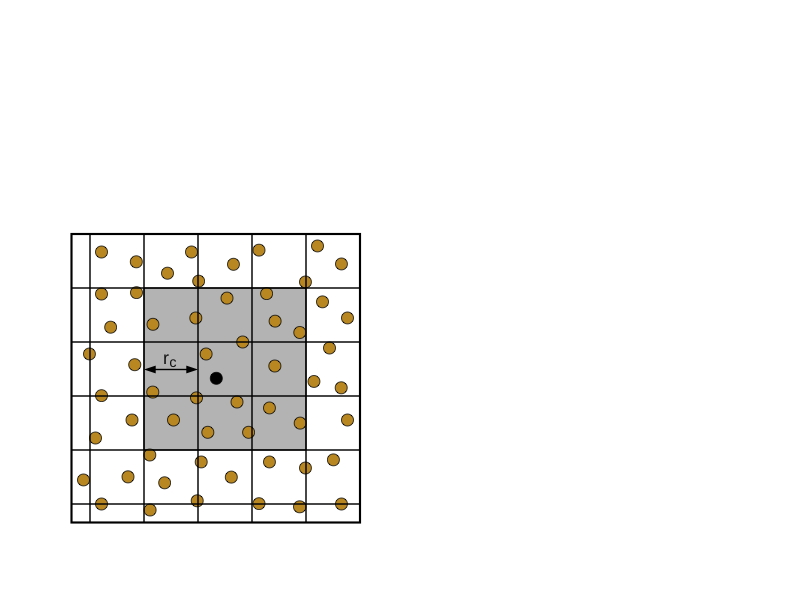
\includegraphics[clip=true,viewport=70 70 362  362,scale=.5]{mdchapter/fig-nb-cell}
} \qquad
\subfigure[Verlet neighbor list method.]{
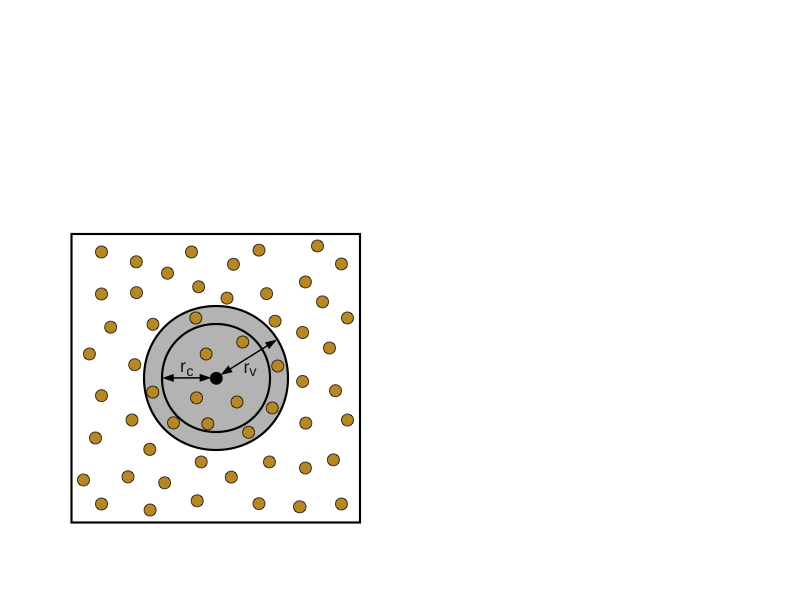
\includegraphics[clip=true,viewport=70 70 362  362,scale=.5]{mdchapter/fig-nb-verlet}
}
\caption{Computing nonbonded forces within a cutoff, $r_c$.  To compute 
forces involving the highlighted particle, only particles in the shaded
regions are considered.}
\label{fig:nb}
\end{center}
\end{figure}

\Level 2 {Cell Lists}  
The idea of cell lists appears often in problems where a
set of points that are nearby a given point is sought.  Referring to
Fig.~\ref{fig:nb}(a), where we illustrate the idea with a 2-D example, a grid is laid
over the set of particles.  If the grid spacing is no less than $r_c$,
then to compute the forces on particle $i$, only the particles in the
cell containing $i$ and the 8 adjacent cells need to be considered.
One sweep through all the particles is used to construct a list of
particles for each cell.  These cell lists are used to compute the forces
for all particles.  At the next time step, since the particles have moved,
the cell lists must be regenerated or updated.  The complexity of this
approach is $O(n)$ for computing the data structure and $O(n \times n_c)$
for the force computation, where $n_c$ is the average number of particles
in 9 cells (27 cells in 3-D).  The storage required for the cell list
data structure is $O(n)$.

\Level 2 {Verlet Neighbor Lists}  
The cell list structure is somewhat
inefficient because, for each particle $i$, $n_c$ particles are
considered, but this is much more than the number of particles within
the cutoff $r_c$.  A Verlet neighbor list is a list of particles within
the cutoff for a particle $i$.  Each particle has its own list, and thus
the storage required is $O(n \times n_v)$ where $n_v$ is the average
number of particles within the cutoff.  Once these lists are constructed,
computing the forces is then very fast, requiring the minimal complexity
$O(n \times n_v)$.  Constructing the list is more expensive, requiring
examining all the particles for each particle, i.e., no less than the
original complexity of $O(n^2)$.  The advantage, however, is that the
neighbor lists can be reused for many time steps if an expanded cutoff,
$r_v$ is used.  Referring to a 2-D example in Fig.~\ref{fig:nb}(b),
the neighbor list can be reused as long as no particle from outside
the two circles moves inside the inner circle.  If the maximum speed
of the particles can be estimated or bounded, then one can determine a
number of time steps for which it is safe to reuse the neighbor lists.
(Alternatively, it may be possible to signal when any particle crosses
to a position within the cutoff.)  Technically, the Verlet neighbor list
is the list of particles within the expanded cutoff, $r_v$.

\Level 2 {Using Cell and Neighbor Lists Together}  
The hybrid approach is simply to use Verlet neighbor
lists but to use cell lists to construct the neighbor lists.  This reduces
the high cost when neighbor lists need to be regenerated.  This hybrid approach
is very effective and is often the approach used in state-of-the-art 
molecular dynamics software.

Both cell lists and Verlet neighbor lists can be modified to exploit the fact
that the force $f_{ij}$ on particle $i$ due to particle $j$ is
equal to $-f_{ji}$ (Newton's third law) and only needs to be
computed once.  For example, for cell lists,
only 4 of the 8 cells (in 2-D) need to be considered.

\Level 1 {Computing Long-Range Forces}

Electrostatic forces are challenging to compute because they are
long-range:  each particle feels a non-negligible electrostatic force
from all other particles in the simulation.  An approximation that is
sometimes used is to truncate the force calculation for a particle after
a certain cutoff radius (as is done for short-range van der Waals forces).
This generally produces unacceptable artifacts in the results, however.

There are several more accurate methods for speeding up
the computation of electrostatic forces, avoiding the $O(n^2)$
sum over all pairs of $n$ particles.  We briefly outline some of these
methods here.

\Level 2 {Hierarchical N-body Methods}  
Hierarchical N-body methods, including
the Barnes-Hut method and the fast multipole method, are popular for
astrophysical particle simulations, but are typically too costly for the
accuracy required in biomolecular simulations.  In the Barnes-Hut method,
space is recursively divided into 8 equal cells (in 3-D) until each
cell contains zero or one particles.  Forces between nearby particles
are computed individually, as normal, but for distant particles, forces
are computed between one particle and a set of distant particles within
a cell.  An accuracy measure is used to determine if the force can
be computed using a distant cell or must be computed by individually
considering its children cells.  The Barnes-Hut method has complexity
$O(n \log n)$.  The fast multipole method has complexity
$O(n)$; this method calculates the potential and does not calculate forces directly.

\Level 2 {Particle-Mesh Methods}  
In particle-mesh methods, we exploit
the Poisson equation
\[
 \nabla^2 \phi = -\frac{1}{\epsilon} \rho
\]
which relates the potential $\phi$ to the charge density $\rho$, where
$1/\epsilon$ is a constant of proportionality.  To utilize this equation, we
discretize space using a mesh, assign charges to the mesh points, solve
Poisson's equation on the mesh to arrive at the potential on the mesh.
The force is the negative gradient of the potential (for conservative
forces such as electrostatic forces).  A number of techniques have been
developed for distributing point charges in space to a set of mesh points
and also for numerically interpolating the force on the
point charges due to the potentials at the mesh points.  Many fast methods
are available for solving the Poisson equation, including multigrid
methods and fast Fourier transforms.  With respect
to terminology, particle-mesh methods are in contrast to the naive {\em
particle-particle} method where forces are computed between all pairs
of particles.

It turns out that particle-mesh methods are not very accurate,
and a more accurate alternative is to split each force into a short-range,
rapidly-varying part and a long-range, slowly-varying part:
\[
f_{ij} = f_{ij}^{sr} + f_{ij}^{lr} .
\]
One way to accomplish this is to weigh $f$ by a function $h(r)$,
which emphasizes the short-range part (small $r$) and by $1-h(r)$ which
emphasizes the long-range part (large $r$).  The short-range part is
computed by computing the interaction of all pairs of particles
within a cutoff (a particle-particle method) and the long-range part
is computed using the particle-mesh method.  The resulting method,
called particle-particle-particle-mesh (PPPM, or P$^3$M) is due to
Hockney and Eastwood, in a series of papers beginning in 1973.

\Level 2 {Ewald Method}  
The Ewald method is the most popular of the methods
described so far for electrostatic forces in biomolecular simulations and
was developed for the case of periodic boundary conditions.  The structure
of the method is similar to PPPM in that the force is split
between short-range and long-range parts.  Again, the short-range part is
computed using particle-particle methods, and the long-range part is
computed using Fourier transforms.  Variants of the Ewald method are
very similar to PPPM in that the long-range part uses a mesh, and fast
Fourier transforms are used to solve the Poisson equation on the mesh.
For additional details, see, for example \cite{frenkel-smit}.  
In Section \ref{sec:fft}, we describe the
parallelization of the 3-D FFT to solve the 3-D Poisson equation.

\Level 0 {Parallel Decompositions}

We now discuss the parallel computation of forces.  Plimpton
\cite{plimpton} created a very useful categorization of molecular dynamics
parallelization methods, identifying {\em atom}, {\em force}, and {\em spatial} 
decomposition
methods.  Here, we closely follow his description of these methods.
We also add a fourth category which has come to be recognized as
differing from the earlier categories, called {\em neutral territory} methods,
a name coined by Shaw \cite{shaw}.  Neutral territory methods are currently
used by many state-of-the-art molecular dynamics codes.
Spatial decompositions and neutral territory methods are particularly
advantageous for parallelizing cutoff-based calculations.

\Level 1 {Atom Decompositions}

In an atom decomposition, each particle is assigned to one processor,
and that processor is responsible for computing the particle's forces and
updating its position for the entire simulation.  For the computation
to be roughly balanced, each processor is assigned approximately the same
number of particles (a random distribution works well).  An important point
of atom decompositions is that each
processor generally needs to communicate with all other processors to
share updated particle positions.

\begin{figure}[htbp]
\begin{center}
\subfigure[Force matrix.]{
%\includegraphics[clip=true,viewport=124 218 505 595,scale=.5]{mdchapter/fig-atom1pdf}
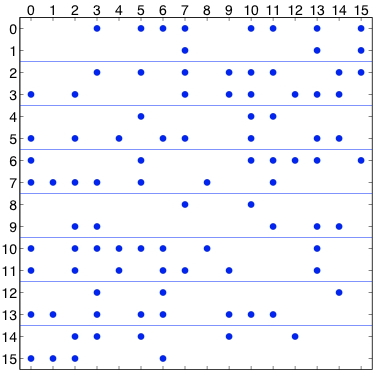
\includegraphics[scale=.5]{mdchapter/fig-atom1v}
}
\subfigure[Force matrix, redundancies removed.]{
%\includegraphics[clip=true,viewport=124 218 505 595,scale=.5]{mdchapter/fig-atom2pdf}
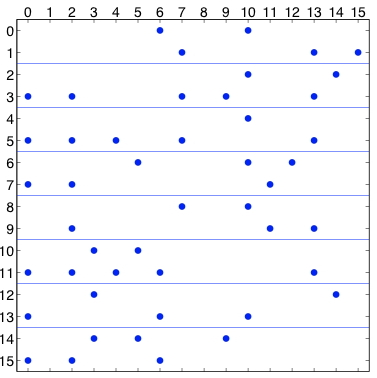
\includegraphics[scale=.5]{mdchapter/fig-atom2v}
}
\caption{Atom decomposition, showing a force matrix of 16 particles
distributed among 8 processors.  A dot represents a nonzero entry in
the force matrix.
On the left, the matrix is symmetric; on the right, only one element of a pair
of skew-symmetric elements is computed, to take advantage of Newton's third law.} 
\label{fig:atom} 
\end{center} 
\end{figure}

An atom decomposition is illustrated by the {\em force matrix} in
Fig.~\ref{fig:atom}(a).  For $n$ particles, the force matrix is an $n$-by-$n$
matrix; the rows and columns are numbered by particle indices.  A nonzero
entry $f_{ij}$ in the matrix denotes a nonzero force on particle $i$
due to particle $j$ which must be computed.  This force may be a nonbonded
and/or a bonded force.  When cutoffs are used, the matrix is sparse, as
in this example.  The matrix is dense if forces are computed between all
pairs of particles.  The matrix is skew-symmetric because of Newton's 
third law, $f_{ij} = -f_{ji}$.
The lines in Fig.~\ref{fig:atom}(a) show how the particles are
partitioned.  In the figure, 16 particles are partitioned among
8 processors.

Algorithm \ref{alg:atom1} shows one time step from the point of view of
one processor.  At the beginning of the time step,
each processor holds the positions of particles assigned to it.
\begin{algorithm}
\caption{Atom decomposition time step.}
\label{alg:atom1}
\begin{algorithmic}[1]
\STATE send/receive particle positions to/from all other processors
\STATE (if nonbonded cutoffs are used) determine which nonbonded forces need to be computed
\STATE compute forces for particles assigned to this processor
\STATE update positions (integration) for particles assigned to this processor
\end{algorithmic}
\end{algorithm}

An optimization is to halve the amount of computation, which is possible because the
force matrix is skew-symmetric.  To do this, we choose
exactly one of $f_{ij}$ or $f_{ji}$ for all skew-symmetric pairs such that each
processor is responsible for computing approximately the same number of
forces.  Choosing the upper or lower triangular part of the force matrix
is a bad choice because the computational load is unbalanced.  A better
choice is to compute $f_{ij}$ if $i+j$ is even in the upper triangle, or
if $i+j$ is odd in the lower triangle, as shown in Fig.~\ref{fig:atom}(b).
There are many other options.

When taking advantage of skew-symmetry in the force matrix,
all the forces on a particle owned by a processor are no longer computed
by that processor.  For example, in Fig.~\ref{fig:atom}(b), the forces
on particle 1 are no longer computed only by the first processor.  
To complete the force calculation,
processors must communicate to send forces that are needed by other
processors and receive forces that are computed by other processors.
The above algorithm must now be modified by adding a communication
step (step 4) as shown in Algorithm \ref{alg:atom2}.
\begin{algorithm}
\caption{Atom decomposition time step, without redundant calculations.}
\label{alg:atom2}
\begin{algorithmic}[1]
\STATE send/receive particle positions to/from all other processors
\STATE (if nonbonded cutoffs are used) determine which nonbonded forces need to be computed
\STATE compute {\em partial} forces for particles assigned to this processor
\STATE send particle forces needed by other processors and receive particle forces needed by this processor
\STATE update positions (integration) for particles assigned to this processor
\end{algorithmic}
\end{algorithm}

This algorithm is advantageous if the extra communication is outweighed by
the savings in computation.  Note that the amount of communication doubles
in general.

\Level 1 {Force Decompositions}

In a force decomposition, the forces are distributed among the processors
for computation.  A straightforward way to do this is to partition
the force matrix into blocks and to assign each block to a processor.
Fig.~\ref{fig:force}(a) illustrates this for the case of 16 particles
and 16 processors.  
Particles also need to be assigned to processors (as in atom decompositions)
for the purpose of having processors assigned to update particle positions.
In the example of the Figure, processor $i$ is assigned to update the
positions of particle $i$; in practical problems, a processor would 
be assigned to update the positions of many particles.
Note that, again, we first consider the case of a skew-symmetric
force matrix.  

\begin{figure}[htbp]
\begin{center}
\subfigure[Force matrix.]{
%\includegraphics[clip=true,viewport=124 218 505 595,scale=.5]{mdchapter/fig-force1pdf}
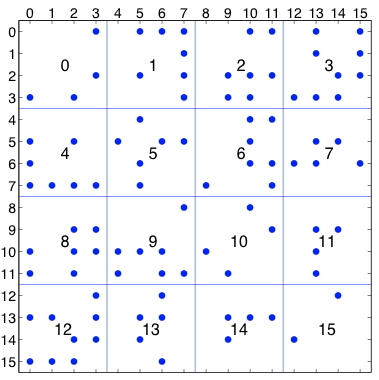
\includegraphics[scale=.5]{mdchapter/fig-force1v}
}
\subfigure[Force matrix, redundancies removed.]{
%\includegraphics[clip=true,viewport=124 218 505 595,scale=.5]{mdchapter/fig-force1sympdf}
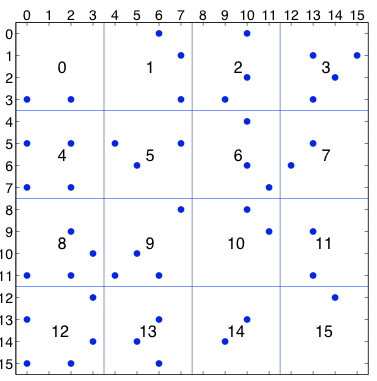
\includegraphics[scale=.5]{mdchapter/fig-force1symv}
}
\caption{Force decomposition, showing a force matrix of 16 particles and 
forces partitioned among 16 processors.}
\label{fig:force}
\end{center}
\end{figure}

We now examine the communication required in a time step
for a force decomposition.  Consider processor 3, which computes partial forces for
particles 0, 1, 2, 3, and needs positions from particles 0, 1, 2, 3, and
also 12, 13, 14, 15.  Thus processor 3 needs to perform communication with
processors 0, 1, 2, 3, and processors 12, 13, 14, 15.  After forces have
been computed by all processors, processor 3 needs to collect forces
on particle 3 computed by other processors.  Thus processor 2 needs to perform
communication again with processors 0, 1, 2, 3.

Algorithm \ref{alg:force1} shows what is performed in one time step,
from the point-of-view of one processor.
At the beginning of the time step, each processor
holds the positions of all the particles assigned to it.
\begin{algorithm}
\caption{Force decomposition time step.}
\label{alg:force1}
\begin{algorithmic}[1]
\STATE send positions of my assigned particles which are needed by
other processors; receive {\em row} particle positions needed by my processor
(this communication is between processors in the same processor row, e.g., processor
3 communicates with processors 0, 1, 2, 3)
\STATE receive {\em column} particle positions needed by my processor
(this communication is generally with processors in another processor row, e.g.,
processor 3 communicates with processors 12, 13, 14, 15)
\STATE (if nonbonded cutoffs are used) determine which nonbonded forces need to be computed
\STATE compute forces for my assigned particles
\STATE send forces needed by other processors; receive forces needed for my
assigned particles (this communication is between processors in the same 
processor row, e.g., processor 3 communicates with processors 0, 1, 2, 3)
\STATE update positions (integration) for my assigned particles
\end{algorithmic}
\end{algorithm}

In general, if there are $p$ processors (and $p$ is square, for simplicity),
then the the force matrix is partitioned into $\sqrt{p}$ by $\sqrt{p}$ blocks.
The force decomposition just described requires a processor to communicate
in three steps, with $\sqrt{p}$ processors in each step.  This is much 
more efficient than atom decompositions which require communications among all
$p$ processors.

We can also exploit Newton's third law in force decompositions.
Like for atom decompositions, we first choose a modified force matrix
where only one of $f_{ij}$ and $f_{ji}$ is computed.  The forces
on particle $i$ are computed by a row of processors and now also by
a column of processors.  Thus an extra step of communication is needed
by each processor to collect forces from a column of processors
for particles assigned to it.  
Whereas there were three
communication steps, there are now four communication steps when
Newton's third law is exploited (the communication is not doubled
in this case as in atom decompositions).

A modification to the force decomposition saves some communication.
In Fig.~\ref{fig:force-perm}, the columns are reordered using a 
{\em block-cyclic} ordering.  Consider again processor 3, which computes
partial forces for particles 0, 1, 2, 3.  It needs positions from
particles 0, 1, 2, 3, as before, but now also with processors 3, 7,
11, 15.  The latter are processors in the same processor column as
processor 3.  Thus all communications are within the same processor row
or processor column, which may be advantageous on mesh-based network
architectures.  The modified method is shown as
Algorithm \ref{alg:force2}.

\begin{figure}[htbp]
\begin{center}
\subfigure[Force matrix.]{
%\includegraphics[clip=true,viewport=124 218 505 595,scale=.5]{mdchapter/fig-force2pdf}
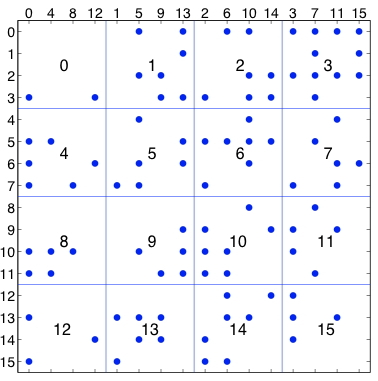
\includegraphics[scale=.5]{mdchapter/fig-force2v}
}
\subfigure[Force matrix, redundancies removed.]{
%\includegraphics[clip=true,viewport=124 218 505 595,scale=.5]{mdchapter/fig-force2sympdf}
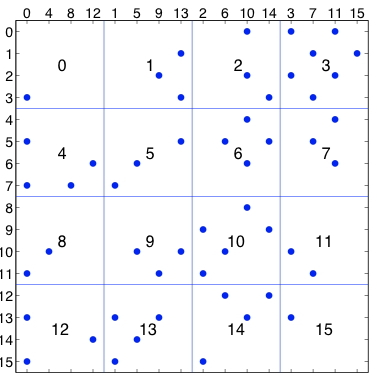
\includegraphics[scale=.5]{mdchapter/fig-force2symv}
}
\caption{Force decomposition, with permuted columns in the force matrix.
Note that columns 3, 7, 11, 15 are now in the block column corresponding to
processors 3, 7, 11, 15 (the same indices), etc.}
\label{fig:force-perm}
\end{center}
\end{figure}

\begin{algorithm}
\caption{Force decomposition time step, with permuted columns of force matrix.}
\label{alg:force2}
\begin{algorithmic}[1]
\STATE send positions of my assigned particles which are needed by
other processors; receive {\em row} particle positions needed by my processor
(this communication is between processors in the same processor row, e.g., processor
3 communicates with processors 0, 1, 2, 3)
\STATE receive {\em column} particle positions needed by my processor
(this communication is generally with processors the same processor column, e.g.,
processor 3 communicates with processors 3, 7, 11, 15)
\STATE (if nonbonded cutoffs are used) determine which nonbonded forces need to be computed
\STATE compute forces for my assigned particles
\STATE send forces needed by other processors; receive forces needed for my
assigned particles (this communication is between processors in the same 
processor row, e.g., processor 3 communicates with processors 0, 1, 2, 3)
\STATE update positions (integration) for my assigned particles
\end{algorithmic}
\end{algorithm}

\Level 1 {Spatial Decompositions}

In a spatial decomposition, space is decomposed into cells.
Each cell is assigned to a processor which is responsible
for computing the forces on particles that lie inside the cell.
Fig.~\ref{fig:spatial}(a) illustrates a spatial decomposition into 64 cells for the
case of a 2-D simulation.  (This is a decomposition of space and is
not to be confused with a force matrix.)  Typically, the number of cells
is chosen to be equal to the number of processors.
Since particles move during
the simulation, the assignment of particles to cells changes as well.
This is in contrast to atom and force decompositions.

Fig.~\ref{fig:spatial}(b) shows one cell (center square) and the region of space (shaded)
that contains particles that are potentially within the cutoff radius, $r_c$, with particles in 
the given cell.  The shaded region is often called the {\em import region}, since 
the given cell must import positions of particles lying in this region to 
perform its force calculation.  Note that 
not all particles in the given cell must interact with all particles in the import
region, especially if the import region is large compared to the cutoff radius.

\begin{figure}[htbp]
\begin{center}
\subfigure[Decomposition into 64 cells.]{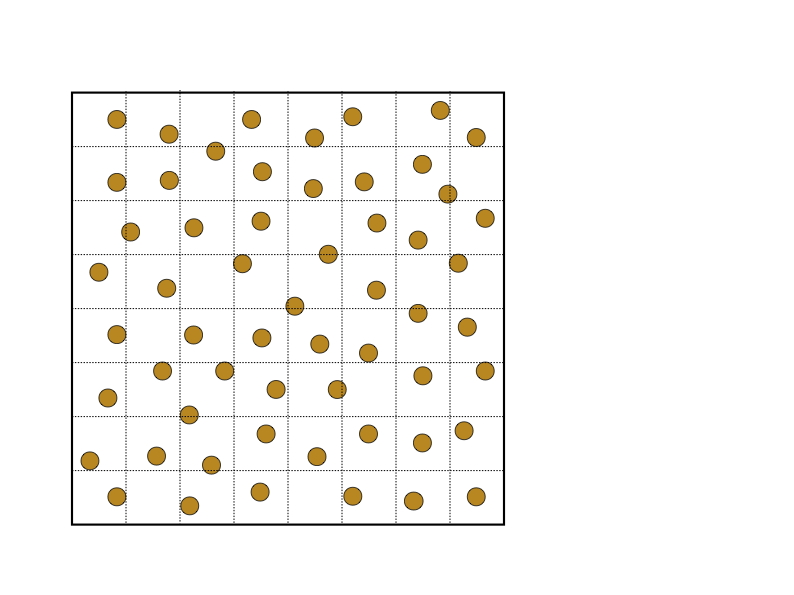
\includegraphics[clip=true,viewport=70 70 506 506,scale=.40]{mdchapter/fig-spatial1}} \qquad
\subfigure[Import region for one cell.]{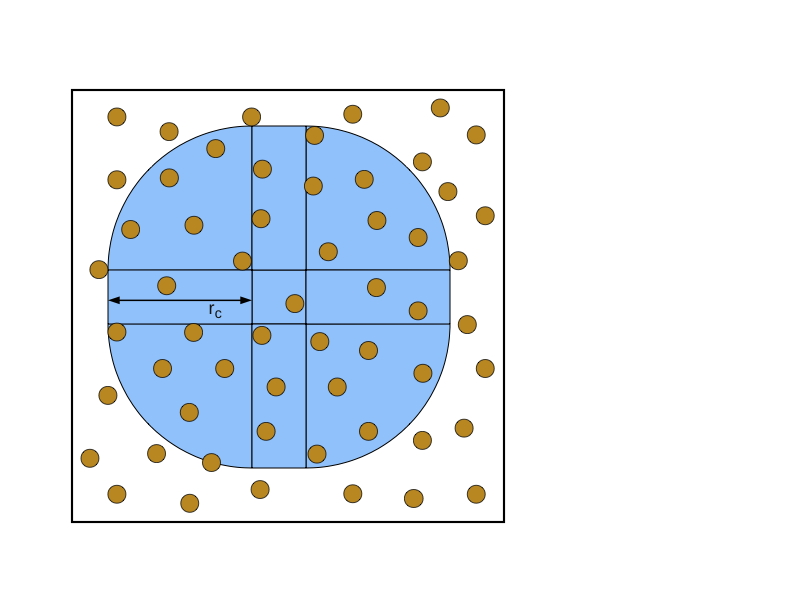
\includegraphics[clip=true,viewport=70 70 506 506,scale=.40]{mdchapter/fig-spatial2}}
\caption{Spatial decomposition, showing particles in a 2-D computational box, (a) partitioned into
64 cells, (b) import region for one cell.}
\label{fig:spatial}
\end{center}
\end{figure}

Algorithm \ref{alg:spatial} shows what each processor performs in one time step.
We assume that at the beginning of the time step, each processor holds the positions
of the particles in its cell.
\begin{algorithm}
\caption{Spatial decomposition time step.}
\label{alg:spatial}
\begin{algorithmic}[1]
\STATE send positions needed by other processors for particles in their import regions;
receive positions for particles in my import region
\STATE compute forces for my assigned particles
\STATE update positions (integration) for my assigned particles
\end{algorithmic}
\end{algorithm}

To exploit Newton's third law, the shape of the import region can be halved.
Now each processor only computes a partial force on particles in its cell, and 
needs to receive forces from other processors to compute the total force
on these particles.  Thus an extra step of communication is involved.
We leave it as an exercise to the reader to work out the details of the
modified import region and the pseudocode for this case.

In the implementation of a spatial decomposition method, each cell is
associated with a list of particles in its import region, similar to a 
Verlet neighbor list.  Like a Verlet neighbor list, it is not necessary
to update this list at every time step, if the import region is expanded
slightly.  This allows the import region list to be reused for several
time steps, corresponding to the amount of time it takes a particle 
to traverse the width of the expanded region.  This is exactly analogous
to Verlet neighbor lists.

In summary, the main advantage of spatial decomposition methods is
that they only require communication between processors corresponding
to nearby particles.  A disadvantage of spatial decomposition methods
is that, for very large numbers of processors, the import region
is large compared to the number of particles contained inside each cell.

\Level 1 {Neutral Territory Methods}

Our description of neutral territory methods follows closely
that of Shaw \cite{shaw}.  
A neutral territory method can be viewed as combining aspects of
spatial decompositions and force decompositions.  To parallelize
the integration step, particles are assigned to processors 
according to a partitioning of space.  To parallelize the 
force computation, each processor computes the forces between
two sets of particles, but these particles may be unrelated
to the particles that have been assigned to the processor for
integration.  As a result of this additional flexibility,
neutral territory methods may require much less communication
than spatial decomposition methods.

An example of a neutral territory method is shown in Fig.~\ref{fig:nt}
for the case of a 2-D simulation.
In the method shown in the Figure, the given processor is assigned
the computation of forces between particles lying in the horizontal
bar with particles lying in the vertical bar.  These two regions thus
form the import region for this method.  By comparing to Fig.~\ref{fig:nt}(b),
the import region for this neutral territory method is much smaller
than that for the corresponding spatial decomposition method.
The advantage is greater when the size of the cells corresponding to
each processor is small compared to the cutoff radius.

\begin{figure}[htb]
\begin{center}
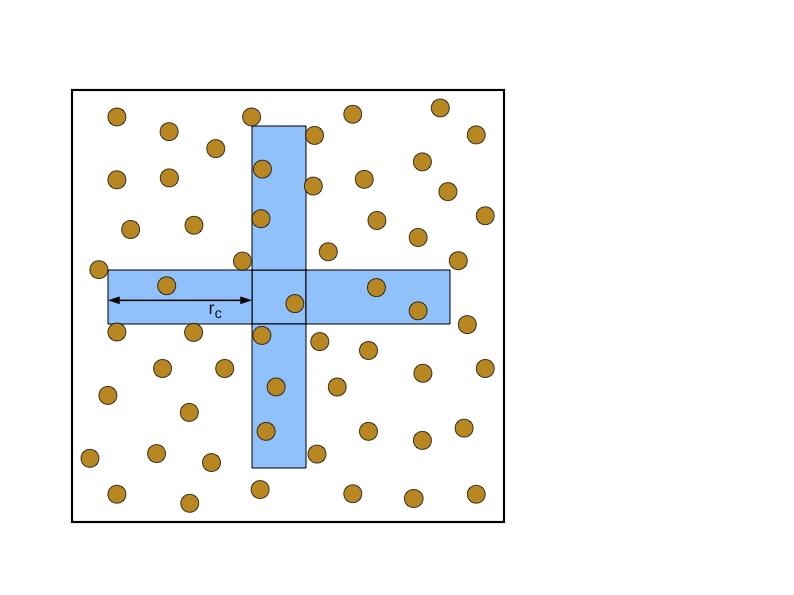
\includegraphics[clip=true,viewport=70 70 506 506,scale=.40]{mdchapter/fig-ntmethod}
\caption{Neutral territory method, showing particles in a 2-D computational box
and the import region (shaded) for one cell (center square).  This Figure can
be compared directly to the spatial decomposition case of Fig.~\ref{fig:spatial}(b).
See Shaw \cite{shaw} for additional details.}
\label{fig:nt}
\end{center}
\end{figure}

After the forces are computed, the given processor sends the forces
it has computed to the processors that need these forces for integration.
We thus have Algorithm \ref{alg:nt}.
\begin{algorithm}
\caption{Neutral territory method time step.}
\label{alg:nt}
\begin{algorithmic}[1]
\STATE send and receive particle positions corresponding to import regions
\STATE compute forces assigned to this processor
\STATE send and receive forces required for integration
\STATE update positions (integration) for particles assigned to this processor
\end{algorithmic}
\end{algorithm}

Like other methods, the import region of the neutral territory method can 
be modified to take advantage of Newton's third law.  We refer to
Shaw \cite{shaw} for additional details and for illustrations of neutral
territory methods in 3-D simulations.

\Level 0 {Parallel Fast Fourier Transform}
\label{sec:fft}

A common component of many methods for computing long-range forces
is the 3-D FFT for solving the Poisson equation on a 3-D mesh.
The Fourier transform diagonalizes the Poisson operator (called 
the Laplacian) and one
forward and one inverse FFT transformation are required in 
the solution.  Consider the discrete Laplacian operator $L$
(with periodic boundary conditions)
and the solution of $\phi$ in $-L \phi = \rho$.  Let $F$ denote
the Fourier transform.  The original problem is equivalent to
\begin{eqnarray*}
 - (F L F^{-1}) F \phi & = &  F \rho \\
 \phi & = & - F^{-1} (F L F^{-1})^{-1} F \rho .
\end{eqnarray*}
The matrix $F L F^{-1}$ is diagonal.  The forward Fourier transform
$F$ is applied to $\rho$, then the Fourier-space components are scaled
by the inverse of the diagonal matrix, and finally, the inverse
Fourier transform $F^{-1}$ is applied to obtain the solution $\phi$.

For realistic protein sizes, a mesh spacing of approximately 1 {\AA}ngstrom
is typically used, leading to a 3-D mesh that is quite small by many
standards:  $64 \times 64 \times 64$, or $128 \times 128 \times 128$.  
Parallel computation would often
not be applied to a problem of this size, but parallel computation must
be used because the data $\rho$ is already distributed among the parallel
processors (assuming a spatial decomposition is used).

A 3-D FFT is computed by computing 1-D FFTs in sequence along each of the
three dimensions.  For the $64 \times 64 \times 64$ mesh size, this is 4096 1-D
FFTs of dimension 64.  The parallel FFT calculation is typically bound
by communication.  The best parallelization of the FFT depends on the
size of the transforms and the architecture of the computer network.
Below, we first describe some concepts for parallel 1-D FFTs and then
describe some concepts for parallel 3-D FFTs.  For current software and
research dedicated to the parallelization and efficient computation
(using SIMD operations)
of large 1-D transforms, we refer to the SPIRAL and FFTW packages.
These packages use autotuning to generate FFT codes that are efficient
for the user's computer architecture.

\Level 1 {Parallel 1-D FFT}

\Level 2 {1-D FFT without Transpose}
Fig.~\ref{fig:fft1} shows the data dependencies (data flow diagram)
between the inputs (left) and outputs (right) for the 16-point radix-2
decimation-in-frequency FFT algorithm.  (Not shown is a bit-reversal
permutation that may be necessary in the computation.)  The Figure
also shows a partitioning of the computation among four processors.
In this parallelization, the initial data is not moved among processors,
but communication occurs during the computation.  In the example shown in
the Figure, communication occurs in the first two FFT stages; the final
two stages do not involve communication.  When communication does occur,
every processor communicates with exactly one other processor.

\Level 2 {1-D FFT with Transpose}
Use of transposes is common to parallelize FFT computations.
Fig.~\ref{fig:fft2}(a) shows the same data flow diagram as in
Fig.~\ref{fig:fft1}, but horizontal lines have been removed and additional
index labels have been added for clarity.  As before, the first two FFT
stages are performed without communication.  The data is then transposed
among the processors.  With this transposed data layout, the last two
FFT stages can be performed without communication.  The final data is
not in the original order; an additional transpose may be needed, or the
data may be used in this transposed order.  Fig.~\ref{fig:fft2}(b) shows
how the indices are partitioned among four processors before and after
the transpose.  From these two Figures, notice that the first two stages
have data dependencies that only involve indices in the same partition.
The same is true for the second two stages for the partitioning after
the transpose.  Observe also that the structure of the computations
before and after the transpose are identical.

\begin{figure}[htbp]
\begin{center}
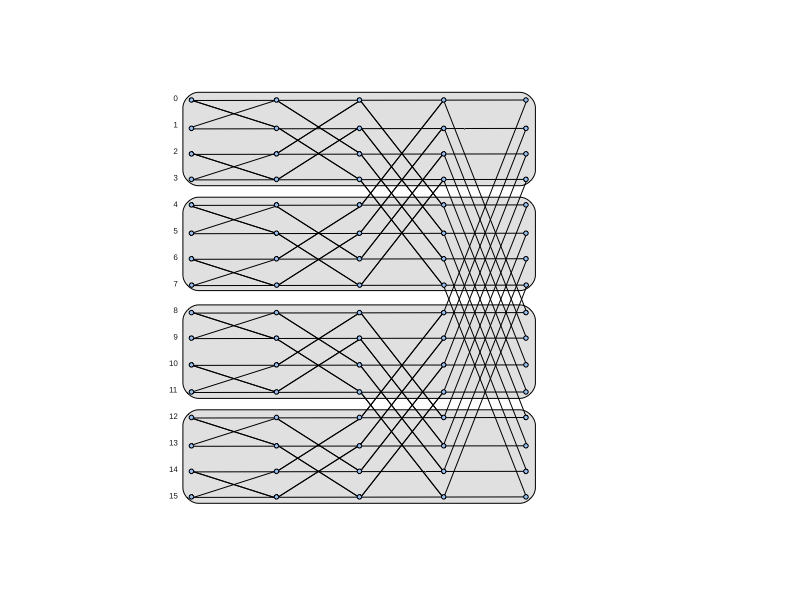
\includegraphics[clip=true,viewport=144 85 576 540,scale=.5]{mdchapter/fig-fft-first}
\caption{Data flow diagram for 1-D FFT for 16 points.  The shaded
regions show a decomposition for 4 processors (one processor per region).
In this parallelization, 
the first two FFT stages have no communication; the last two FFT stages
do have communication.}
\label{fig:fft1}
\end{center}
\end{figure}

\begin{figure}[htb]
\begin{center}
\subfigure[Data flow diagram (shown without horizontal lines for clarity) for 1-D FFT for 16 points.]{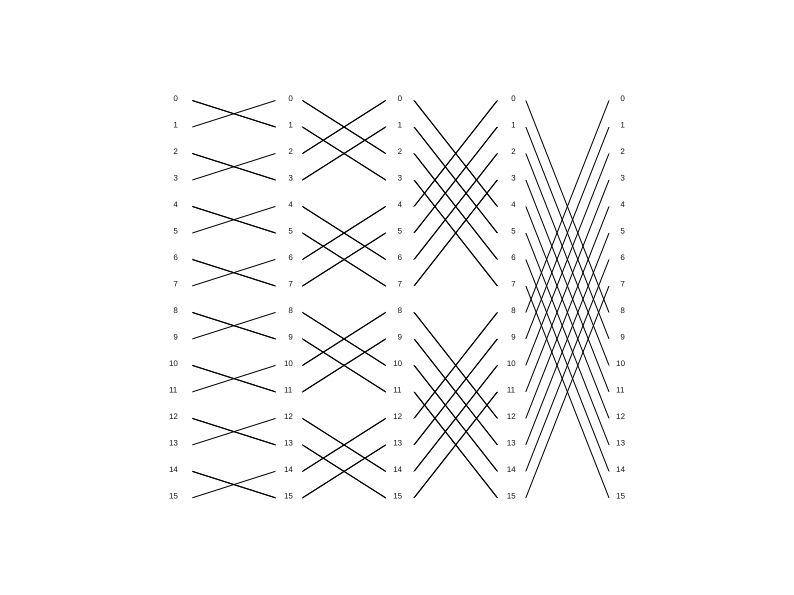
\includegraphics[clip=true,viewport=144 85 648 522,scale=.5]{mdchapter/fig-fft-second}} \quad
\subfigure[Partitioning of the indices before (left) and after (right) the transpose.]{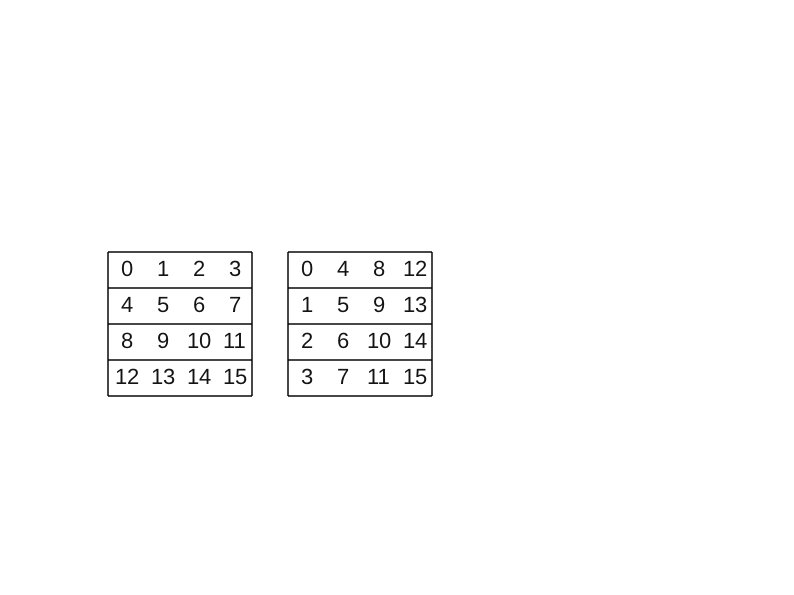
\includegraphics[clip=true,viewport=100 190 436 360,scale=.3]{mdchapter/fig-fft-third}}
\caption{1-D FFT with transpose.  The first two stages do not involve communication.  The data is then transposed among the processors.  As a result, the second two stages also do not involve communication.}
\label{fig:fft2}
\end{center}
\end{figure}

\Level 1 {Parallel 3-D FFT}

\Level 2 {3-D FFT with Block Decomposition}  
Fig.~\ref{fig:fft3}(a) shows a block decomposition of the FFT input
data when a spatial decomposition is used for a mesh of size $8~\times
8~\times 8$ distributed across 64 processors arranged in a $4~\times
4~\times 4$ topology.  The parallel 1-D FFT algorithms can be applied in
each of the dimensions.  For the example shown in the Figure, each 1-D
FFT computation involves 4 processors.  Each processor performs multiple
1-D FFTs simultaneously (four in this example).  Within each processor,
data is ordered contiguously if traversing one of the dimensions, and
thus data access is strided for computation in the other two dimensions.
Strided data access can be slow, and thus it may be worthwhile to reorder
the data within each processor when computing the FFT for each of the dimensions.

\Level 2 {3-D FFT with Slab Decomposition}  
The slab decomposition is shown in 
Fig.~\ref{fig:fft3}(b) for the case of 4 processors.  Each processor holds
one or more planes of the input data.  This decomposition is used if
the input data is already distributed in slabs, or if it can be 
redistributed this way.  The two 1-D FFTs in the plane of the slabs
require no communication.  The remaining 1-D FFTs require communication
and could use one of the two approaches for parallel 1-D FFTs described above.  
A disadvantage
of the slab decomposition is that for large numbers of processors, the
number of processors may exceed the number of points in the 3-D FFT along
any one dimension.  An alternative is the pencil decomposition below.

\Level 2 {3-D FFT with Pencil Decomposition}  
The pencil decomposition
is shown in Fig.~\ref{fig:fft3}(c) for the case of 16 processors.
Each processor holds one or more pencils of the input data.  If the
original input data is distributed in blocks as in Fig.~\ref{fig:fft3}(a),
then communication among a row of processors (in a 3-D processor mesh)
can distribute the data into the pencil decomposition.  The 1-D FFTs
can then be performed with no communication.  To perform the 1-D FFT in
another dimension, the data needs to be redistributed into pencils in
another dimension.  In total, four communication stages are needed for
the entire 3-D FFT computation.

\begin{figure}[htbp]
\begin{center}
\subfigure[Block Decomposition]{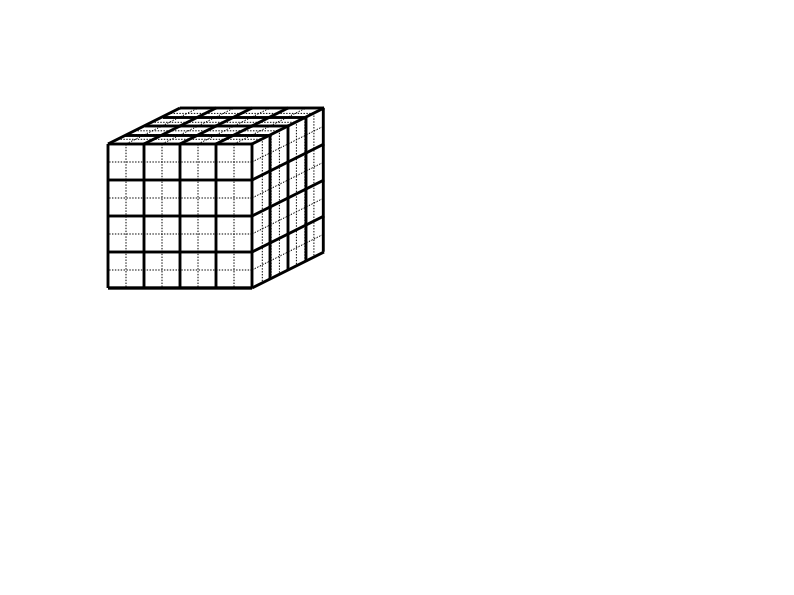
\includegraphics[clip=true,viewport=100 300 330 490,scale=.6]{mdchapter/fig-fft1}}% \quad
\subfigure[Slab Decomposition]{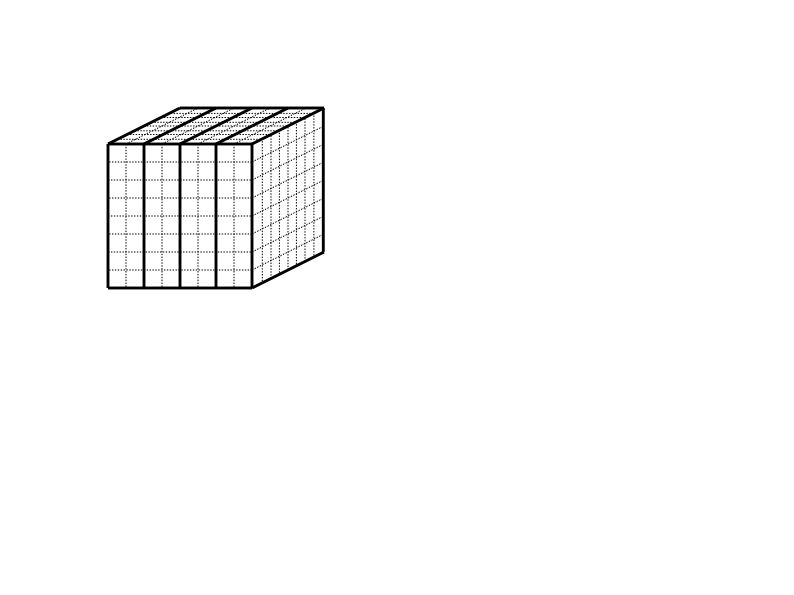
\includegraphics[clip=true,viewport=100 300 330 490,scale=.6]{mdchapter/fig-fft2}}% \quad
\subfigure[Pencil Decomposition]{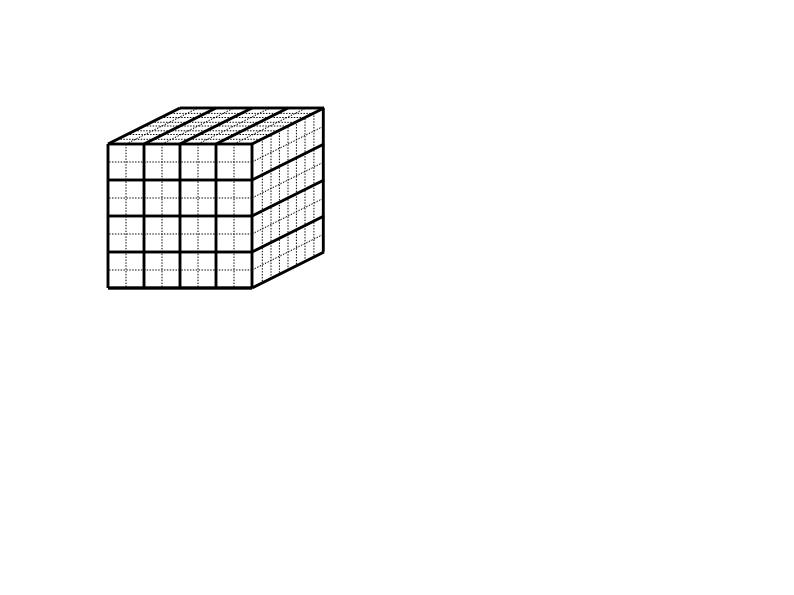
\includegraphics[clip=true,viewport=100 300 330 490,scale=.6]{mdchapter/fig-fft3}}
\caption{Three data decompositions for 3-D FFTs.}
\label{fig:fft3}
\end{center}
\end{figure}

\Level 0 {Integration for Molecular Dynamics}

To numerically integrate the system of ordinary differential
equations in molecular dynamics, special methods are required,
different than the traditional ODE solvers that were studied in
Chapter 4.  These special methods, called symplectic methods,
are better than other methods at producing solutions that have
constant energy, for example, for systems that are called
Hamiltonian (which include systems from molecular dynamics).  
When Hamiltonian systems are integrated with many time steps
over a long time interval, preservation of structure such as
total energy is often more important than the order of accuracy
of the method.  In this section, we motivate some ideas and
give some details of the St\"{o}rmer-Verlet method, which is sufficient
for simple molecular dynamics simulations.

Hamiltonian systems are a class of dynamical systems
which conserve energy and which can be written in a form
called Hamilton's equations.  Consider, for symplicity, the {\em simple
harmonic oscillator}
\[
u'' = -u
\]
where $u$ is the displacement of a single particle from an equilibrium
point.  This equation could model a particle with unit mass on a spring
with unit spring constant.  The force on a particle at position $u$ is
$-u$.
This system does not look like a molecular dyanamics system but
is useful for illustrating several ideas.

The above second order equation can be written
as a system of first order equations
\begin{eqnarray*}
q' &=& p \\
p' &=& -q 
\end{eqnarray*}
where $q = u$ and $p=u'$ which is common notation used
in classical mechanics.  The general solution is
\[
\left( \begin{array}{c} q \\ p \end{array} \right)
=
\left( \begin{array}{rr}  \cos t & \sin t \\
                         -\sin t & \cos t \end{array} \right)
\left( \begin{array}{c} q \\ p \end{array} \right) .
\]
The kinetic energy of the simple harmonic oscillator is
$p^2/2$ and the potential energy is $q^2/2$ (the negative 
gradient of potential energy is the force, $-q$).
Thus the total energy is proportional to
$q^2 + p^2$.

Now consider the solution of the system of first order equations
by three methods, explicit Euler, implicit Euler, and a method
called the St\"{o}rmer-Verlet method.  The initial condition is $(q,p) = (1,0)$.
We use a time step of $h=0.05$ and
take 500 steps.  We plot $q$ and $p$ on the horizontal and
vertical axes, respectively (called a {\em phase plot}).  The 
exact solution, as given above, is a unit circle centered
at the origin.

Figure~\ref{fig:integ} shows the solutions.  For explicit Euler,
the solution spirals outward, meaning the displacement and 
momentum of the solution increases over time.  The opposite is
true for the implicit Euler method.  A plot of the total energy
would show the energy increasing and decreasing for the two
cases, respectively.  The solutions are better when smaller time
steps are taken or when higher order methods are used, but
these methods are not at all appropriate 
for integration of symplectic systems over long periods of time.
Figure~\ref{fig:integ}(c) shows the solution using a symplectic
method called the St\"{o}rmer-Verlet
method.  The solution shows that $q^2 + p^2$ is preserved much
better than in the other two methods.

\begin{figure}[htbp]
\begin{center}
\subfigure[Explicit Euler]{
%\includegraphics[clip=true,viewport=117 215 499 589,scale=.35]{mdchapter/fig-integ1pdf}
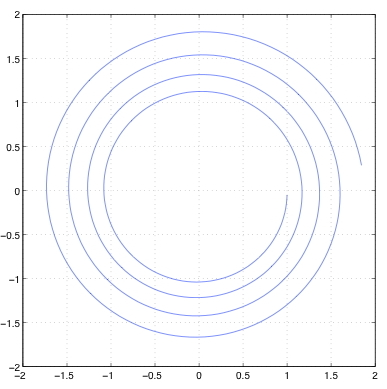
\includegraphics[scale=.35]{mdchapter/fig-integ1v}
}
\subfigure[Implicit Euler]{
%\includegraphics[clip=true,viewport=117 215 499 589,scale=.35]{mdchapter/fig-integ2pdf}
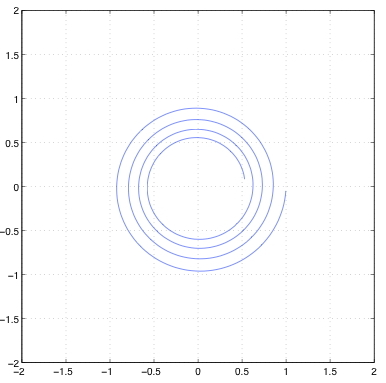
\includegraphics[scale=.35]{mdchapter/fig-integ2v}
}
\subfigure[St\"{o}rmer-Verlet Method]{
%\includegraphics[clip=true,viewport=117 215 499 589,scale=.35]{mdchapter/fig-integ3pdf}
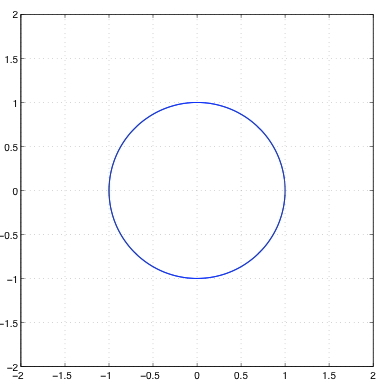
\includegraphics[scale=.35]{mdchapter/fig-integ3v}
}
\caption{Phase plot of the solution of the simple harmonic oscillator for
three methods with initial value (1,0), time step 0.05, and 500 steps.  
For explicit Euler, the solution
spirals outward; for implicit Euler, the solution spirals inward; 
the total energy is best preserved with the St\"{o}rmer-Verlet method.}
\label{fig:integ}
\end{center}
\end{figure}

We derive it 
the St\"{o}rmer-Verlet method for the second order
equation
\[
u'' = f(t, u)
\]
by simply replacing the left-hand side with a finite difference approximation
\[
\frac{u_{k+1} - 2 u_k + u_{k-1}}{h^2} = f(t_k, u_k)
\]
which can be rearranged to obtain the method
\[
u_{k+1} = 2 u_k - u_{k-1} + h^2 f(t_k, u_k) .
\]
The formula can equivalently be derived from Taylor series.
%which shows that it is locally fourth order.  
The method is similar to linear multistep methods in that
some other technique is needed to supply the initial step of the method.  
The method is also time-reversible, because the formula is the same
if $k+1$ and $k-1$ are swapped.
To explain why this method is symplectic, 
unfortunately, is beyond the scope of this introduction.

The method as written above has a number of disadvantages, the most severe being
that the addition of the small $h^2$ term is subject to catastrophic cancellation.
Thus this formula should not be used in this form, and a number of mathematically
equivalent formulas (which can be derived from the formula above) have been developed.

One alternative formula is the {\em leap-frog} method:
\begin{eqnarray*}
u_{k+1} & = & u_k + h v_{k+1/2} \\
v_{k+1/2} & = & v_{k-1/2} + h f(t_k, u_k)
\end{eqnarray*}
where $v$ is the first derivative (velocity) which is offset from
the displacement $u$ by a half step.  This formula does not 
suffer from the same roundoff problems and also makes available the velocities,
although they need to be re-centered with displacements in order to calculate
total energy at a given step.
The second of this pair of equations is basically a finite difference formula.
%with truncation error $O(h^2)$ 

A third form of the St\"{o}rmer-Verlet method is the {\em velocity Verlet}
variant:
\begin{eqnarray*}
u_{k+1} & = & u_k + h v_k + \frac{h^2}{2} f(t_k, u_k) \\
v_{k+1} & = & v_k + \frac{h^2}{2} (f(t_k, u_k) + f(t_{k+1}, u_{k+1}))
\end{eqnarray*}
where now the velocities are computed at the same points as the 
displacements.  Each of these algorithms can be implemented such
that only two sets of quantities need to be stored (two previous positions,
or a position and a velocity).
These variants of the St\"{o}rmer-Verlet method are popular because of
their simplicity, requiring only one costly force evaluation per step.
Higher-order methods have generally not been practical.

The velocity Verlet scheme is also the basis of multiple time
step algorithms for molecular dynamics.  In these algorithms, the
slowly-varying (typically long-range) forces are evaluated less frequently
and update the positions less frequently than the quickly-varying
(typically short-range) forces.  Finally, many state-of-the-art molecular
dynamics integrate a Hamiltonian system that has been modified
in order to control the simulation temperature and pressure.  Much more
complicated symplectic methods have been developed for these systems.

